\section{Research Methodology }

\subsection{Research Approach}
\par The planned approach for this research is a combined approach using \textbf{Action research and mixed methods}.
\newline
Action research is suitable for this research because we plan to use iterative cycles of action, observations, and the participatory nature of the research. Participants feedback and information will continuously refine the emotion baseline recognition system, ensuring the research addresses practical challenges and generates actionable knowledge.(figure \ref{fig:action})
\newline 
The mixed-methods approach integrates quantitative data with qualitative insights, providing a comprehensive evaluation of the framework's effectiveness. Quantitative data will be used to train and validate the machine learning model, while qualitative feedback will offer deeper insights into the participants' experiences and the system's practical applicability. 

\begin{figure*}[h]
\centering
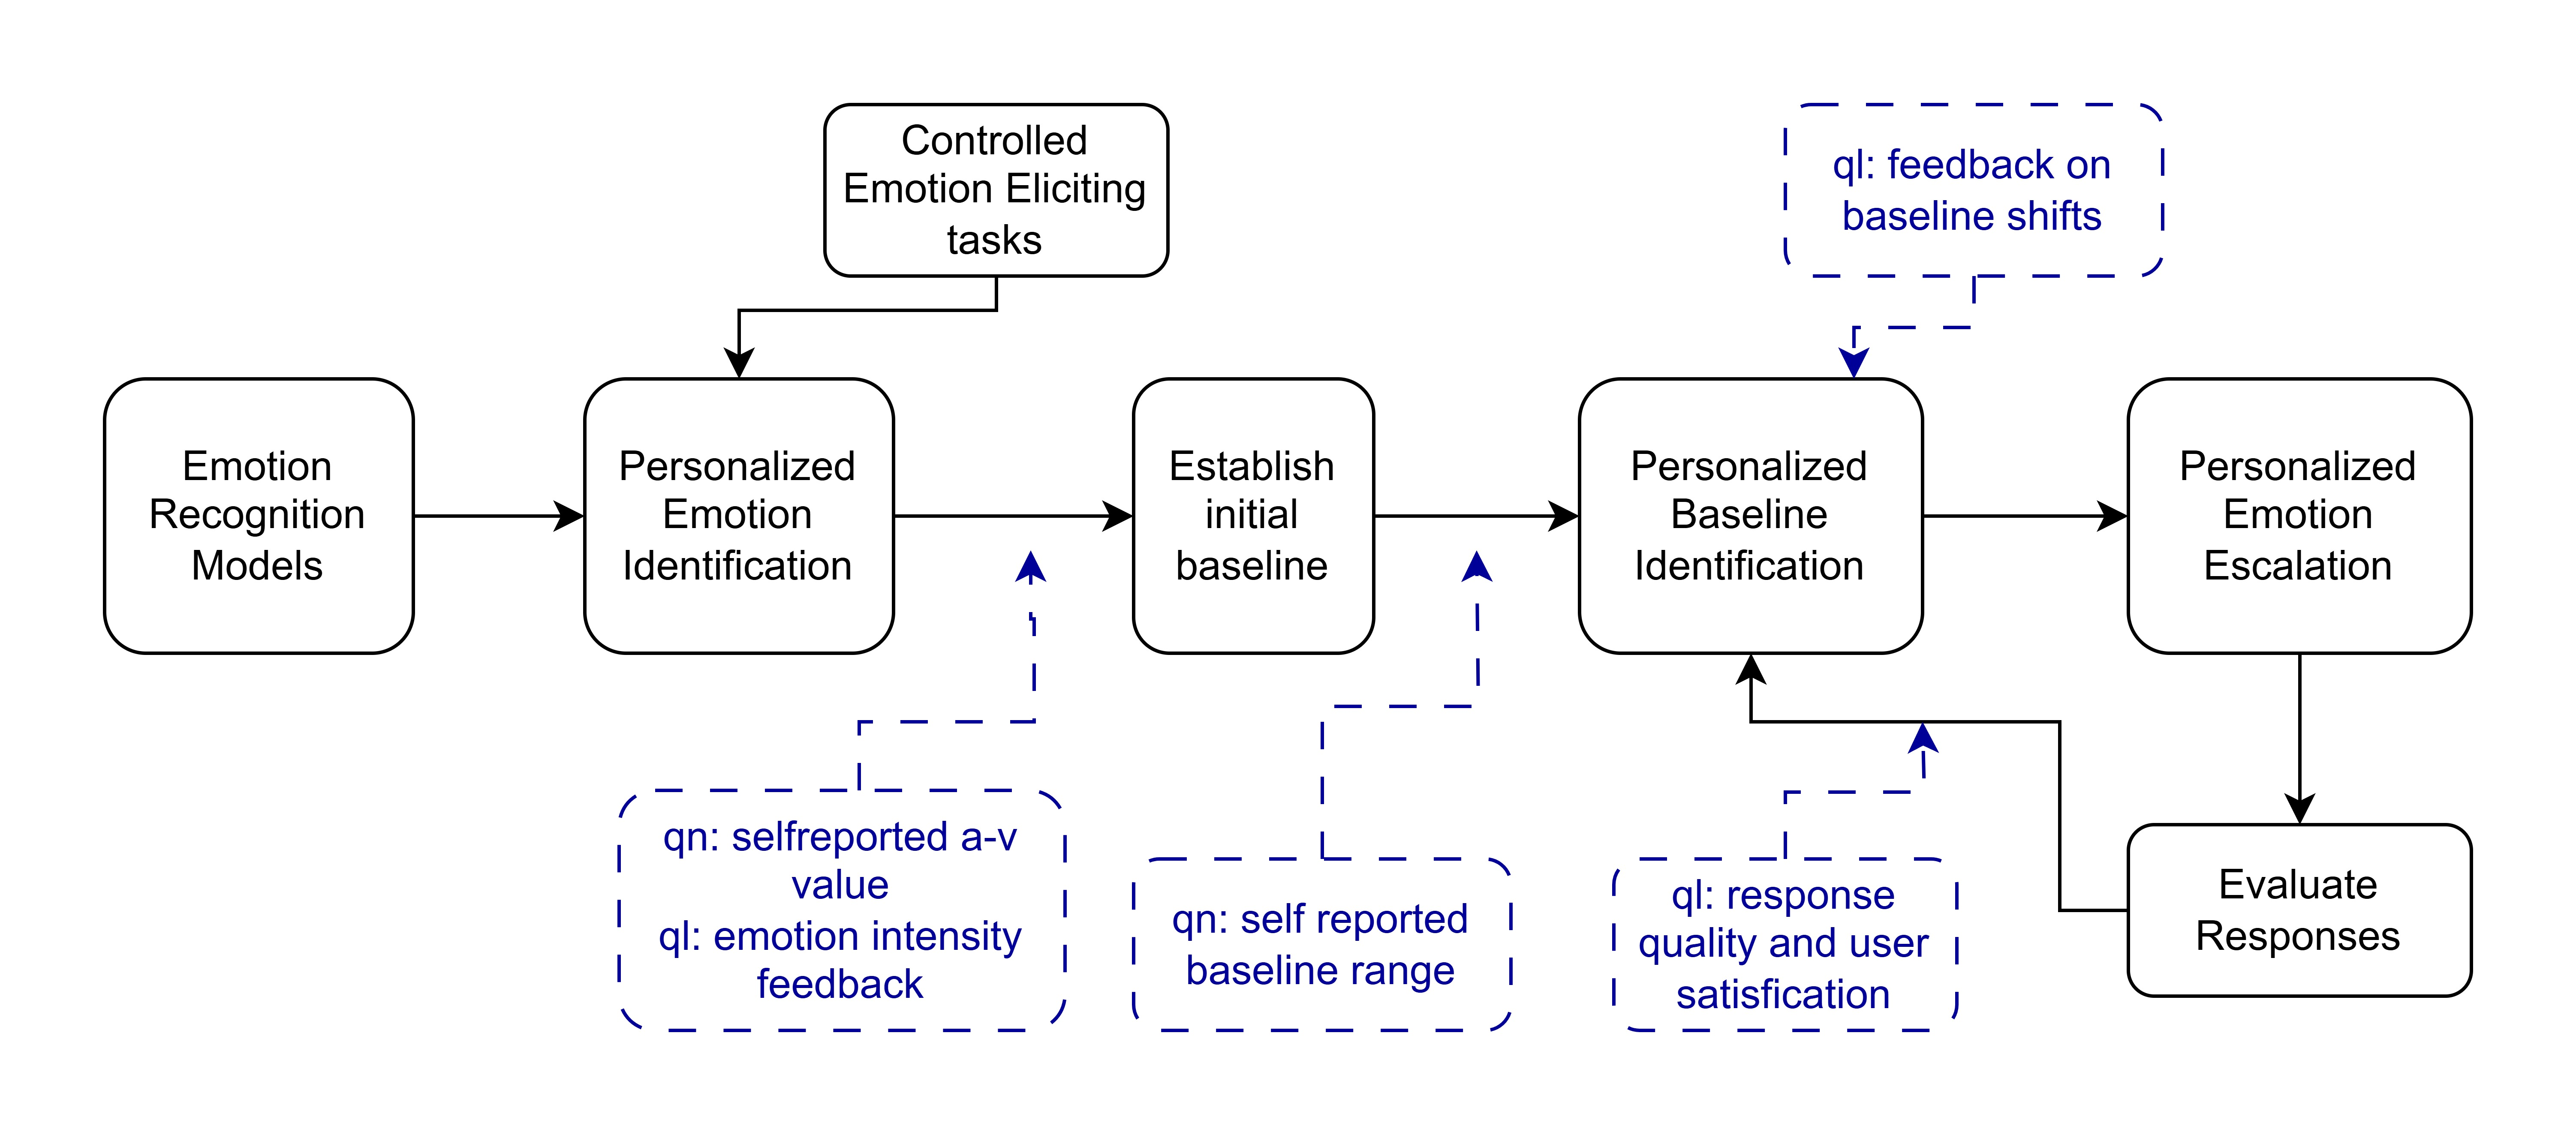
\includegraphics[width=1\textwidth]{img/chapter_01/action-plan.jpg}
\captionof{figure}{Action Plan}
\label{fig:action}
\end{figure*}